% vim:spell spelllang=sk
%\subsection{Signal processing - digitálne filtre}
\section{Signal processing - digitálne filtre}
%% {{{ uvod
Digitálne filtre sú dôležitou súčasťou spracovania digitálneho
signálu. Podobne ako analógové filtre, ich úlohou je zo vstupného
signálu vybrať pre nás podstatnú časť, prípadne ju zosilniť alebo inak
modifikovať signál. V~tomto dokumente si spomenieme niekoľko 
najzákladnejších filtrov používaných v~praxi a~súvisiacich s~Fourierovou
transformáciou. Budeme ich demonštrovať na spracovaní obrazu, hoci
mnohé z~nich sú viac dôležité v~spracovaní zvuku/elektrického signálu 
%\footnote{V elektronickej prílohe je možné nájsť aj demonštráciu 
%týchto filtrov pre zvuk, v publikovanej podobe z pochopiteľných
%dôvodov nie je.}
.

Najskôr si popíšeme filtre pracujúce vo frekvenčnom rozsahu, potom
spomenieme filtre pracujúce na priestorovej doméne a~kapitolu
zavŕšime ukázaním súvisu medzi týmito dvoma prístupmi 
a~dekonvolúciou, ktorá sa snaží invertovať následky nežiadúcich filtrov.
%% }}}

%\subsubsection{Ideálny lowpass a highpass filter}
\subsection{Ideálny lowpass a highpass filter}

Najjednoduchšími filtrami, s~ktorými sa čitateľ môže stretnúť sú
takzvaný lowpass a~highpass filter. Ako už ich názov napovedá, budú
prepúšťať len určité pásmo frekvencií. Lowpass filter prepustí všetky
nízke frekvencie, vysoké odstráni. Príkladom lowpass filtra môže byť
napríklad ekvalizér, keď si necháme iba "basy". Highpass filter je
pravým opakom lowpass filtra - prepustí len vysoké tóny. Príkladom
môže byť aplikácia highpass filtra na obrázok - ponechá iba hrany,
t.j. miesta, kde sa rýchlo mení intenzita obrazu a teda obsahujú
vysoké frekvencie.

Ideálny lowpass a~highpass filter o~limitujúcej frekvencii $f$ môžeme
popísať obrázkom \ref{fig:ideal_lowpass_filter}, 
kde na $x$-ovej osi je frekvencia
vstupného signálu a~na $y$-ovej osi je hodnota výstupného signálu.
\begin{poznamka}
    Väčšina filtrov vo frekvenčnej oblasti sa dá popísať podobným grafom.
    Čitaťeľ ale musí brať ohľad na istú nepresnosť - daný graf
    nešpecifikuje presne filter. Špecifikuje len zmenu amplitúdy.
    Bežné filtre fázu nemenia a~preto sa ticho predpokladá $\phi(f)=0$.
\end{poznamka}

Dané filtre prepúšťajú všetky frekvencie na jednu stranu od hraničnej
a~na druhú stranu neprepustia nič. Ako si ukážeme vizuálne, tieto
filtre majú spoločný problém - "zvonenie". Najvýraznejšie sa prejavuje
práve pri highpass filtri. Preto sa v~praxi nepoužívajú.
Zvonenie úzko súvisí s~Gibbsovým fenoménom, ktorý sme už skúmali
v~kapitole \ref{section:gibbs}. Ideálny lowpass filter je totiž variant čiastočného súčtu
Fourierovho radu prenesený na diskrétnu Fourierovu transformáciu. Pri filtroch
nás teda okrem ich frekvenčnej odozvy bude zaujímať aj "priestorová"
odozva na jednoduchý impulz, ktorým je v~diskrétnom prípade jednotkový
bod. V~spojitom prípade je to Diracova delta funkcia\footnote{
Diracova delta funkcia spĺňa $\forall a>0: \int_{-a}^a \delta(x) \dd x
= 1$. Delta funkcia nie je funkciou v pravom slova zmysle.
Zjednodušene, $\delta(x)=0$ ak $x\not=0$ a $\delta(0)=\infty$.
}. Kombinovaním grafu pre
frekvenčnú odozvu a~zodpovedajúceho grafu pre priestorovú odozvu
sa môžeme presvedčiť o~vlastnostiach filtra. Dobrý filter by
mal mať rýchly úpadok pri prechode cez hraničnú frekvenciu,
zároveň by však nemal vykazovať prvky zvonenia v~priestorovej doméne.

% {{{ fig:ideal_lowpass
\begin{figure}[htp]
    \def\path{obrazky/informatika/digitalne_filtre}
    \centering
    \subfigure[Frekvenčná odozva]{
        \includegraphics{\path/ideal_lowpass_frequency_10}
        \includegraphics{\path/ideal_lowpass_frequency_20}
        \includegraphics{\path/ideal_lowpass_frequency_40}
    }
    \subfigure[Priestorová odozva]{
        \includegraphics{\path/ideal_lowpass_response_10}
        \includegraphics{\path/ideal_lowpass_response_20}
        \includegraphics{\path/ideal_lowpass_response_40}
    }
    \subfigure[Aplikácia filtra]{
        \includegraphics{\path/ideal_lowpass_10}
        \includegraphics{\path/ideal_lowpass_20}
        \includegraphics{\path/ideal_lowpass_40}
    }
    \caption{Ideálny lowpass filter pre $f=10,20,40$}
    \label{fig:ideal_lowpass_filter}
\end{figure}
% }}}

Na obrázku \ref{fig:ideal_lowpass_filter} môžeme nájsť
frekvenčnú odozvu filtra, jeho priestorovú odozvu na bodový impulz 
a~ukážku filtrovania obrazu. Je dôležité si všimnúť najmä zvonenie 
v~priestorovej odozve a~následný dopad na kvalitu obrazu. Obrázok má
rozlíšenie $256\cross256$ a~sú naň postupne aplikované filtre o~hraničnej
frekvencii\footnote{Pri diskrétnej transformácii
frekvencia 1 zodpovedá sínusovému signálu o~perióde dĺžky obrázku}
10,20,40.

Ideálny highpass filter bude mať presne opačnú odozvu ako ideálny
lowpass filter. Viac všeobecne, môžeme hovoriť, že frekvenčná odozva
highpass filtra je
\begin{equation}
    f_H(\omega) = 1 - f_L(\omega)
    \label{eq:highpass_filter}
\end{equation}
Pretože súčet oboch filtrov dodáva pôvodný obraz, je ihneď zjavné že
aj ideálny highpass filter bude mať podobné zvoniace efekty ako jeho
brat. Jeho charakteristika sa dá nájsť na obrázku
\ref{fig:ideal_highpass_filter}.

% {{{ fig:ideal_highpass
\begin{figure}[htp]
    \def\path{obrazky/informatika/digitalne_filtre}
    \centering
    \subfigure[Frekvenčná odozva]{
        \includegraphics{\path/ideal_highpass_frequency_10}
        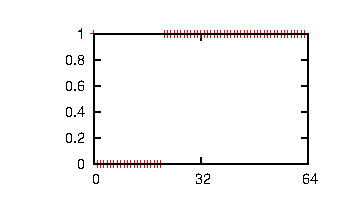
\includegraphics{\path/ideal_highpass_frequency_20}
        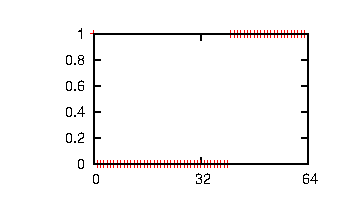
\includegraphics{\path/ideal_highpass_frequency_40}
    }
    \subfigure[Priestorová odozva]{
        \includegraphics{\path/ideal_highpass_response_10}
        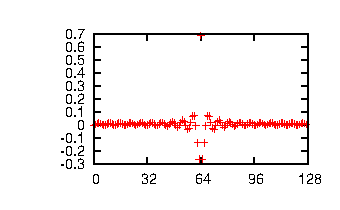
\includegraphics{\path/ideal_highpass_response_20}
        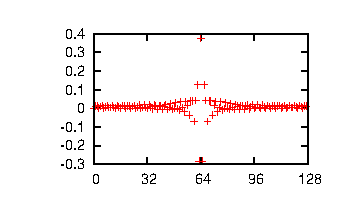
\includegraphics{\path/ideal_highpass_response_40}
    }
    \subfigure[Aplikácia filtra]{
        \includegraphics{\path/ideal_highpass_10}
        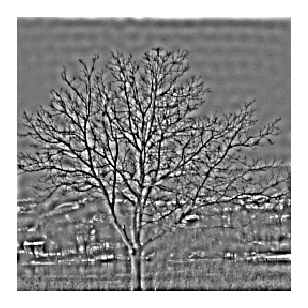
\includegraphics{\path/ideal_highpass_20}
        
\includegraphics{\path/ideal_highpass_40}
    }
    \caption{Ideálny highpass filter pre $f=10,20,40$}
    \label{fig:ideal_highpass_filter}
\end{figure}
% }}}

Pri highpass filtroch ešte spomenieme jednu výnimku rovnice
\eqref{eq:highpass_filter}. Ide konkrétne o~frekvenciu 0, čiže
aritmetický priemer signálu.
Ak počítame výpočty v~hodnotách bez znamienka (0-255), efektívne
vynulovanie rovnicou \eqref{eq:highpass_filter} by spôsobilo posun jasu
k~čiernym farbám. V~tomto prípade je vhodné nastaviť výslednú hodnotu
buď konštantne na polovicu jasu, alebo ponechať pôvodný priemer, čiže
mať jednotkovú odozvu.

%\subsubsection{Hladké filtre}
\subsection{Hladké filtre}
Ako sme v~predchádzajúcej sekcii ukázali, ideálne filtre majú zvoniaci
efekt. Preto sa v~praxi používajú filtre, ktoré majú spojitý a~hladký
prechod medzi frekvenciami, ktoré filtrujú a~frekvenciami, ktoré
nefiltrujú. Ukážeme si dva rôzne filtre - Butterworthov a Gaussov.
Začneme Gaussovým (lowpass) filtrom, ktorý je definovaný rovnicou
\begin{align*}
g_L(f) &= e^{- \frac{1}{2} (\frac{f}{f_0})^2} \\
g_H(f) &= 1 - e^{- \frac{1}{2} (\frac{f}{f_0})^2}
\end{align*}

Gaussov filter je priamym opakom ideálneho filtra. Jeho pozoruhodnou
vlastnosťou je rovnaká hladká podoba vo frekvenčnej a~priestorovej doméne.
Preto ho môžeme považovať akosi za "ideálne hladký" filter. Gaussov
filter sa využíva napríklad na rozmazávanie obrazu.

% {{{ fig:gauss_lowpass
\begin{figure}[htp]
    \def\path{obrazky/informatika/digitalne_filtre}
    \centering
    \subfigure[Frekvenčná odozva]{
        \includegraphics{\path/gauss_lowpass_frequency_10}
        \includegraphics{\path/gauss_lowpass_frequency_20}
        \includegraphics{\path/gauss_lowpass_frequency_40}
    }
    \subfigure[Priestorová odozva]{
        \includegraphics{\path/gauss_lowpass_response_10}
        \includegraphics{\path/gauss_lowpass_response_20}
        \includegraphics{\path/gauss_lowpass_response_40}
    }
    \subfigure[Aplikácia filtra]{
        \includegraphics{\path/gauss_lowpass_10}
        \includegraphics{\path/gauss_lowpass_20}
        \includegraphics{\path/gauss_lowpass_40}
    }
    \caption{Gaussov lowpass filter pre $f=10,20,40$}
    \label{fig:gauss_lowpass_filter}
\end{figure}
% }}}

% {{{ fig:gauss_highpass
\begin{figure}[htp]
    \def\path{obrazky/informatika/digitalne_filtre}
    \centering
    \subfigure[Frekvenčná odozva]{
        \includegraphics{\path/gauss_highpass_frequency_10}
        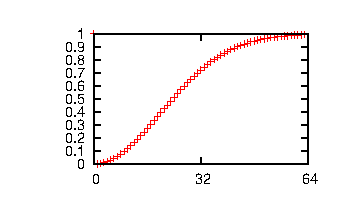
\includegraphics{\path/gauss_highpass_frequency_20}
        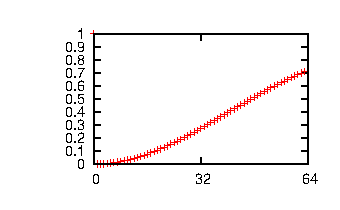
\includegraphics{\path/gauss_highpass_frequency_40}
    }
    \subfigure[Priestorová odozva]{
        \includegraphics{\path/gauss_highpass_response_10}
        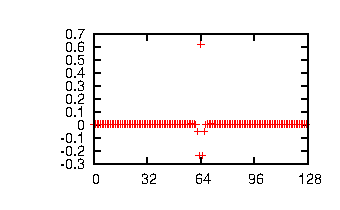
\includegraphics{\path/gauss_highpass_response_20}
        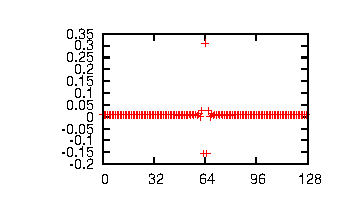
\includegraphics{\path/gauss_highpass_response_40}
    }
    \subfigure[Aplikácia filtra]{
        \includegraphics{\path/gauss_highpass_10}
        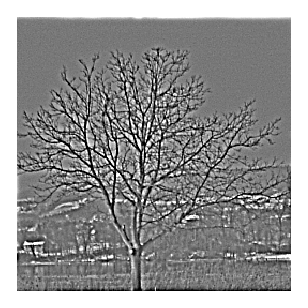
\includegraphics{\path/gauss_highpass_20}
        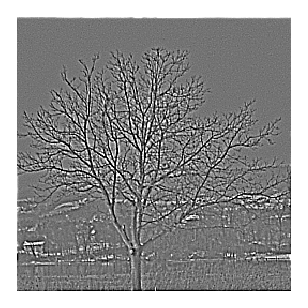
\includegraphics{\path/gauss_highpass_40}
    }
    \caption{Gaussov highpass filter pre $f=10,20,40$}
    \label{fig:gauss_highpass_filter}
\end{figure}
% }}}

Gaussov filter ale tiež nie je ideálne riešenie. Má síce nádhernú
priestorovú odozvu bez zvonenia, jeho frekvenčná odozva je však
pomerne rozťahaná. Prax by preto potrebovala filter bez
zvonenia, ktorý sa ale blíži ideálnemu a~má čo najstrmejší prechod.
Takýmto filtrom je napríklad Butterworthov filter.
Butterworthov filter rádu $n$ s~hraničnou frekvenciou $f_0$
možeme zapísať ako
\begin{align*}
b_L(f) &=  \frac{1}{1 + (\frac{f}{f_0})^{2n}} \\
b_H(f) &= 1- \frac{1}{1 + (\frac{f}{f_0})^{2n}}
\end{align*}
Menením rádu $n$ meníme hladkosť filtra a zároveň jeho zvonenie.
Filtre do rádu $n=2$ majú zvoniaci efekt zanedbateľný, so vzrastajúcim
$n$ ale efekt postupne začína byť čím viac citeľnejší, ako vidieť na
obrázkoch \ref{fig:butterworth_lowpass_filter} a
\ref{fig:butterworth_highpass_filter}.

% {{{ fig:butterworth_lowpass
\begin{figure}[htp]
    \def\path{obrazky/informatika/digitalne_filtre}
    \centering
    \subfigure[Frekvenčná odozva $f=10$]{
        \includegraphics{\path/butterworth_1_lowpass_frequency_10}
        \includegraphics{\path/butterworth_2_lowpass_frequency_10}
        \includegraphics{\path/butterworth_4_lowpass_frequency_10}
    }
    \subfigure[Frekvenčná odozva $f=20$]{
        \includegraphics{\path/butterworth_1_lowpass_frequency_20}
        \includegraphics{\path/butterworth_2_lowpass_frequency_20}
        \includegraphics{\path/butterworth_4_lowpass_frequency_20}
    }
    \subfigure[Frekvenčná odozva $f=40$]{
        \includegraphics{\path/butterworth_1_lowpass_frequency_40}
        \includegraphics{\path/butterworth_2_lowpass_frequency_40}
        \includegraphics{\path/butterworth_4_lowpass_frequency_40}
    }
    \subfigure[Priestorová odozva $f=10$]{
        \includegraphics{\path/butterworth_1_lowpass_response_10}
        \includegraphics{\path/butterworth_2_lowpass_response_10}
        \includegraphics{\path/butterworth_4_lowpass_response_10}
    }
    \subfigure[Priestorová odozva $f=20$]{
        \includegraphics{\path/butterworth_1_lowpass_response_20}
        \includegraphics{\path/butterworth_2_lowpass_response_20}
        \includegraphics{\path/butterworth_4_lowpass_response_20}
    }
    \subfigure[Priestorová odozva $f=40$]{
        \includegraphics{\path/butterworth_1_lowpass_response_40}
        \includegraphics{\path/butterworth_2_lowpass_response_40}
        \includegraphics{\path/butterworth_4_lowpass_response_40}
    }
    \caption{Butterworthov lowpass filter pre rád $n=1,2,4$}
\end{figure}

\begin{figure}[htp]
    \def\path{obrazky/informatika/digitalne_filtre}
    \centering
    \subfigure[Aplikácia filtra $f=10$]{
        \includegraphics{\path/butterworth_1_lowpass_10}
        \includegraphics{\path/butterworth_2_lowpass_10}
        \includegraphics{\path/butterworth_4_lowpass_10}
    }
    \subfigure[Aplikácia filtra $f=20$]{
        \includegraphics{\path/butterworth_1_lowpass_20}
        \includegraphics{\path/butterworth_2_lowpass_20}
        \includegraphics{\path/butterworth_4_lowpass_20}
    }
    \subfigure[Aplikácia filtra $f=40$]{
        \includegraphics{\path/butterworth_1_lowpass_40}
        \includegraphics{\path/butterworth_2_lowpass_40}
        \includegraphics{\path/butterworth_4_lowpass_40}
    }

    \caption{Butterworthov lowpass filter pre rád $n=1,2,4$}
    \label{fig:butterworth_lowpass_filter}
\end{figure}
% }}}

% {{{ fig:butterworth_highpass
\begin{figure}[htp]
    \def\path{obrazky/informatika/digitalne_filtre}
    \centering
    \subfigure[Frekvenčná odozva $f=10$]{
        \includegraphics{\path/butterworth_1_highpass_frequency_10}
        \includegraphics{\path/butterworth_2_highpass_frequency_10}
        \includegraphics{\path/butterworth_4_highpass_frequency_10}
    }
    \subfigure[Frekvenčná odozva $f=20$]{
        \includegraphics{\path/butterworth_1_highpass_frequency_20}
        \includegraphics{\path/butterworth_2_highpass_frequency_20}
        \includegraphics{\path/butterworth_4_highpass_frequency_20}
    }
    \subfigure[Frekvenčná odozva $f=40$]{
        \includegraphics{\path/butterworth_1_highpass_frequency_40}
        \includegraphics{\path/butterworth_2_highpass_frequency_40}
        \includegraphics{\path/butterworth_4_highpass_frequency_40}
    }
    \subfigure[Priestorová odozva $f=10$]{
        \includegraphics{\path/butterworth_1_highpass_response_10}
        \includegraphics{\path/butterworth_2_highpass_response_10}
        \includegraphics{\path/butterworth_4_highpass_response_10}
    }
    \subfigure[Priestorová odozva $f=20$]{
        \includegraphics{\path/butterworth_1_highpass_response_20}
        \includegraphics{\path/butterworth_2_highpass_response_20}
        \includegraphics{\path/butterworth_4_highpass_response_20}
    }
    \subfigure[Priestorová odozva $f=40$]{
        \includegraphics{\path/butterworth_1_highpass_response_40}
        \includegraphics{\path/butterworth_2_highpass_response_40}
        \includegraphics{\path/butterworth_4_highpass_response_40}
    }
    \caption{Butterworthov highpass filter pre rád $n=1,2,4$}
\end{figure}

\begin{figure}[htp]
    \def\path{obrazky/informatika/digitalne_filtre}
    \centering
    \subfigure[Aplikácia filtra $f=10$]{
        \includegraphics{\path/butterworth_1_highpass_10}
        \includegraphics{\path/butterworth_2_highpass_10}
        \includegraphics{\path/butterworth_4_highpass_10}
    }
    \subfigure[Aplikácia filtra $f=20$]{
        \includegraphics{\path/butterworth_1_highpass_20}
        \includegraphics{\path/butterworth_2_highpass_20}
        \includegraphics{\path/butterworth_4_highpass_20}
    }
    \subfigure[Aplikácia filtra $f=40$]{
        \includegraphics{\path/butterworth_1_highpass_40}
        \includegraphics{\path/butterworth_2_highpass_40}
        \includegraphics{\path/butterworth_4_highpass_40}
    }

    \caption{Butterworthov highpass filter pre rád $n=1,2,4$}
    \label{fig:butterworth_highpass_filter}
\end{figure}
% }}}

%\subsubsection{Súvis medzi frekvenčnými a priestorovými filtrami}
\subsection{Súvis medzi frekvenčnými a~priestorovými filtrami}
Klasické obrazové filtre v~priestorovej doméne ako napríklad medián, 
ostrenie hrán a~ich komplikovanejšie verzie vieme popísať ako maticu
$M$ rozmerov $2k+1 \cross 2k+1$ spĺňajúcu
\begin{equation*}
    A_{x,y} = \sum_{i=0}^{2k} \sum_{j=0}^{2k} a_{x+i-k, y+j-k}
    M_{i,j}
\end{equation*}
\begin{poznamka}
    Táto matica vlastne popisuje výslednú hodnotu $A_{i,j}$ ako
    lineárnu kombináciu okolitých bodov $a_{x,y}$. Matica je navyše
    centrovaná aby stred matice zodpovedal bodu, ktorý ostáva na
    mieste.
\end{poznamka}
Pre jednorozmerné signály samozrejme použijeme vektor namiesto matice.
Identita sa dá zapísať ako 
\begin{equation*}
    I = \begin{pmatrix}
            0 & 0 & 0 \\
            0 & 1 & 0 \\
            0 & 0 & 0
        \end{pmatrix}
\end{equation*}
a~filter na detekciu hrán je napríklad
\begin{equation*}
    I = \begin{pmatrix}
            -1/8 & -1/8 & -1/8 \\
            -1/8 & 1 & -1/8 \\
            -1/8 & -1/8 & -1/8
        \end{pmatrix}
\end{equation*}
Filtrovanie v~časovej doméne je pomerne jednoduché a~existuje veľké
množstvo filtrov. Súvislosť s~filtrovaním vo frekvenčnej doméne je
preto veľmi zaujímavým cieľom. Je výhodné vedieť prevádzať filtre
medzi týmito doménami. Užitočným príkladom môže byť napríklad postupná
aplikácia niekoľkých filtrov v~časovej doméne za sebou na jeden obrázok.
Daný výpočet môže byť pomalý, ak sa začnú aplikovať veľké filtre.
Navyše, pri neustálych výpočtoch môže dochádzať k~strate presnosti 
v~dôsledku zaokrúhľovania. Preto je výhodnejšie previesť filtre na ich
frekvenčné dvojčatá a~aplikovať ich vo frekvenčnej doméne.
Už na prvý pohľad výpočet filtra v~časovej doméne matne pripomína
konvolúciu. Túto konvolúciu si teraz explicitne zapíšeme.
\begin{lema}
    Nech $M'$ je matica filtra $M$ "posunutá" do stredu a~preklopená
    podľa oboch osí. Presnejšie, nech 
    \begin{equation*}
        M'_{i,j} = \left\{
            \begin{array}{l l}
               M_{k-i,k-j}, \quad &  -k \le i,j \le k \\
               0, \quad \textit{v ostatných prípadoch}
            \end{array}
            \right.
    \end{equation*}
    Potom aplikácia filtra $M$ je (necyklická) konvolúcia obrazu
    $a$ s~filtrom $M'$.
    \label{lema:filter_konvolucia}
\end{lema}
\begin{dokaz}
    \begin{equation*}
    \begin{split}
        (a * M')_{x,y} &= \sum_i \sum_j a_{i,j} M'_{x-i,y-j} \\
        &= \sum_{\substack{-k\le x-i\\ x-i\le k}}\quad
           \sum_{\substack{-k\le y-j\\y-j\le k}}
           a_{i,j} M_{-x+i+k, -y+j+k} \\
        &= \sum_{\substack{-k\le i-x\\i-x\le k}}\quad
           \sum_{\substack{-k\le j-y\\j-y\le k}}
           a_{i,j} M_{-x+i+k, -y+j+k} \\
        &= \sum_{i=-k+x}^{k+x}
           \sum_{j=-k+y}^{k+y}
           a_{i,j} M_{-x+i+k, -y+j+k} \\
        &= \sum_{r=0}^{2k}
           \sum_{s=0}^{2k}
           a_{r+x-k,s+y-k} M_{-x+(r+x-k)+k, -y+(s+y-k)+k} \\
        &= \sum_{r=0}^{2k}
           \sum_{s=0}^{2k}
           a_{r+x-k,s+y-k} M_{r,s}
    \end{split}
    \end{equation*}
\end{dokaz}
Lema \ref{lema:filter_konvolucia} nám umožňuje prevádzať jednoduché
filtre medzi časovou a~frekvenčnou doménou. Podľa konvolučnej vety
(tabuľka \ref{tab:dft_properties}) je
totiž konvolúcia ekvivalentná jednoduchému násobeniu vo frekvenčnej
doméne. Samozrejme, ak uvažujeme diskrétnu Fourierovu transformáciu,
musíme uvažovať cyklickú konvolúciu. V~praxi to znamená rozšíriť
obrázok a~filter na takú veľkosť, aby súčet ich rozmerov bol menší ako
rozmery Fourierovej transformácie (Napríklad pre filter veľkosti
$5\cross5$ a obrázok veľkosti $100\cross100$ treba použiť Fourierovu
transformáciu o veľkosti aspoň $105\cross105$).
Filtrovanie v~časovej
a~frekvenčnej doméne sa teda opäť prevádza pomocou Fourierovej
transformácie.

%\subsubsection{Gaussov filter verzus iterovaný priemer}
%
%Filtrom "symetrický priemer" nazveme filter, ktorého vektor je $1/4,1/2,1/4$.
%Ide v podstate o filter 
%\begin{equation}
%A_i = \frac{\frac{a_{i-1}+a_i}{2} + \frac{a_i + a_{i+1}}{2}}{2}
%\end{equation}
%Ide o najjednoduchší príklad vyhladzovacieho
%filtra\footnote{Presnejšie povedané najjednoduchší symetrický prípad}.
%Jeho aplikovaní vyhladíme obrázok a stlmíme šum, samozrejme za cenu
%jemného rozmazania hrán. Ak výsledný obrázok stále nie je dostatočne
%hladký, môžeme túto procedúru zopakovať.
%Opakovanou aplikáciou tohoto filtra dostávane filter "iterovaný
%priemer". Cieľom tejto kapitoly je ukázať, že iterovaný priemer sa
%blíži ku Gaussovmu lowpass filtru, ak počet iterácii rastie do
%nekonečna.
%Na obrázku \ref{fig:iterovany_median} máme zobrazený interovaný filter
%s rôznym počtom iterácii.
%\begin{figure}[htp]
%    \centering
%    \includegraphics{obrazky/informatika/signal_processing/iterated_median}
%    \caption{Iterovaný medián}
%    \label{fig:iterated_median}
%\end{figure}
%
%Už z obrázka možno vidieť trend približovaniu sa ku Gaussovej krivke.
%\begin{lema}
%    Vektor iterovaného mediánu po $k$ iteráciach je
%    \begin{equation}
%        IM(k) = \frac{1}{4^k} 
%            (\binom{2k}{0}, \binom{2k}{1}, \binom{2k}{2}, \dots,
%                \binom{2k}{2k})
%    \end{equation}
%    \label{lema:iterated_median}
%\end{lema}
%Z pravdepodobnosti a centrálnej limitnej vety vieme, že postupnosť z
%lemy \ref{lema:iterated_median} konverguje ku Gaussovej krivke.
%Iterovaný medián s dostatočným počtom iterácii je preto Gaussov filter
%v priestorovej doméne. Fourierovou transformáciou Gaussovej krivka je
%ale podľa \todo{} opäť Gaussova krivka.
%To znamená, že iterovaný medián je postupným približovaním sa ku
%Gaussovmu filtru ukazujúc zaujímavú súvislosť medzi vyhladzovaním v
%priestorovej a časovej doméne.

%\subsection{Dekonvolúcia}
\subsection{Dekonvolúcia}

V~niektorých prípadoch má užívateľ na vstupe signál, ktorý bol
upravený konvolúciou. Táto zmena nie je nutne žiadaná. Príkladom môže
byť starý gramofón, ktorý výraznejšie lepšie prehrával zvuk na
svojej rezonančnej frekvencii. Alebo napríklad jemne rozostrená
fotografia, hudba prehrávaná z~pásky atď.
Ďalším príkladom konvolúcie
je napäťový priebeh obdĺžnikového signálu v~reálnych elektrických
obvodoch. Všetky tieto príklady majú spoločný bod - signál z~pôvodnej
(chcenej) podoby prešiel fyzikálnym javom na konvolvovaný. Princíp
dekonvolúcie je preto veľmi jednoduchý - našim cieľom je nájsť filter
rušiaci pôvodnú konvolúciu.
Ak pôvodný signál označíme $x$, konvolvovaný $y$, konvolučný
filter $f$ a~náhodný šum $v$, potom
\begin{equation*}
    y(t) = h(t)*x(t) + v(t)
\end{equation*}
Našou úlohou je nájsť filter $g$ taký, aby
\begin{equation*}
  \hat{x}(t) = g(t)*y(t)
\end{equation*}
kde $\hat{x}$ je odhad $x$ minimalizujúci strednú kvadratickú chybu
$\eps$.

\def\E{{\mathbb{E}}}
\begin{equation*}
\begin{split}
\eps(f) &= \E | X(f) - \hat{X(f)}|^2 \\
        &= \E | X(f) - G(f) Y(f)| ^2 \\
        &= \E | X(f) - G(f) [ H(f) X(f) +V(f)]|^2 \\
        &= \E | [ 1 - G(f) H(f)] X(f) - G(f) V(f)|^2
\end{split}        
\end{equation*}
Roznásobením druhej mocniny dostávame
\begin{equation*}
\begin{split}
\eps(f) =& [1 - G(f) H(f)]\conjug{[1 - G(f) H(f)]} \E| X(f)|^2 \\
  &+ [1-G(f) H(f)]\conjug{G(f)} \E( X(f) \conjug{V(f)}) \\
  &+ G(f) \conjug{[1-G(f)H(F)]} \E( V(f) \conjug{X(f)}) \\
  &+ G(f) \conjug{G(f)} \E|s(f)|^2
\end{split}
\end{equation*}
Predpoklad, že šum je nezávislý od signálu môžeme reprezentovať ako
\begin{equation*}
 \E( X(f)\conjug{V(f)}) = \E(V(f)\conjug{X(f)}) = 0
\end{equation*}
%
Ak si zadefinujeme
\begin{align*}
 S(f) &= \E| X(f)|^2 \\
 N(f) &= \E| V(f)|^2
\end{align*}
Tak dostávame
\begin{equation*}
\eps(f) = [1-G(f)H(f)]\conjug{[1-G(f)H(f)]} S(f)
   + G(f) \conjug{G(f)} N(f)
\end{equation*}
Aby sme našli minimálnu chybu, zderivujeme celú rovnicu podľa $G(f)$ 
a~položíme rovnú nule\footnote{Po správnosti by sa patrilo ešte overiť,
že sme dostali naozaj minimum a nie maximum, toto ale prenecháme na
čitateľa}. Aby sme nemuseli minimalizovať cez 2 premenné (imaginárnu 
a~reálnu časť), pre reálnu funkciu $f$ premennej $z$ existuje skratka:
Ak označíme $z_r = \frac{z + \conjug{z}}{2}, z_i =
\frac{z-\conjug{z}}{2 \imag}$, potom
\begin{equation*}
\pd{f}{\conjug{z}}|_z = 
  \pd{z_r}{\conjug{z}}|_z \pd{f}{z_r}|_{z_i} +
    \pd{z_i}{\conjug{z}}|_z \pd{f}{z_i}|_{z_r} =
 \frac{1}{2} \left(
    \pd{f}{z_r}|_{z_i} + \imag \pd{f}{z_i}|_{z_r}
    \right)
\end{equation*}
Preto na minimalizáciu cez všetky potrebné hodnoty nám stačí položiť
\begin{equation*}
 0 = \pd{f}{\conjug{z}}|_z
\end{equation*}
Aplikovaním na $\eps$ dostávame
\begin{align*}
\d{\eps(f)}{G(f)} &= -\conjug{H(f)} S(f)[1 - G(f) H(f)]  + G(f) N(f) =
0 \\
G(f) &= \frac{\conjug{H(f)} S(f)}{H{f}\conjug{H{f}} S{f} + N{f}}
\end{align*}
Daný dekonvolučný filter sa nazýva Wienerov filter.
Rovnica Wienerovho filtra môže byť ďalej prepísaná do viac vysvetľujúcej podoby
\begin{equation*}
G(f) = \frac{1}{H{f}} 
   \frac{|H(f)|^2}{|H(f)|^2 + \frac{1}{SNR{f}}}
\end{equation*}
kde $SNR{f} = S(f)/N(f)$ je "signal-to-noise ratio", čiže pomer sily
signálu voči šumu. Ak je šum
nulový, člen v~zátvorke je nulový a~dekonvolučný filter je iba
inverzným filtrom. Akonáhle sa ale šum zväčší, člen v~zátvorke sa
zmenší. Wienerov filter preto utlmuje frekvencie na základe ich SNR.

Pre funkčnosť Wienerovho filtra potrebujeme vedieť frekvenčné
charakteristiky jednak signálu a~jednak šumu. Tieto charakteristiky sa
síce nedajú bez pôvodného signálu zistiť presne, v~praxi však často
postačuje približný odhad.

\smalltodo{nejaky obrazok filtra}
\smalltodo{nejaky rozumnejsi zaver?}
\nocite{wiki:wiener}
